\section {Track Jets}
\label{section2}

The tracking systems of ECCE allow for the measurement of lower momentum charged jets with excellent scale and resolution.  The analysis was completed with 18x275 GeV Pythia 8 electron proton collisions, requiring a $Q^2$ greater than $100 \hbox{ GeV}^2$, and the prop.4 detector configuration \cite{ecce-note-comp-2021-02}.  The anti-$k_T$ jet finding algorithm was utilized, with a jet radius $R=0.5$.  To prevent the classification of single particles as jets, a constraint of $z<0.95$ as applied, where 
\begin{equation}
z=\frac{E_{\hbox{most energetic constituent}}}{E_{\hbox{total jet}}}.
\label{eq:jet_z}
\end{equation}

Tracks with a transverse momentum of $p_{T\hbox{, track}} > 30\hbox{ GeV/c}$ are rejected to stay within the limits of the tracking detectors.

\begin{figure}[h]
    \centering
    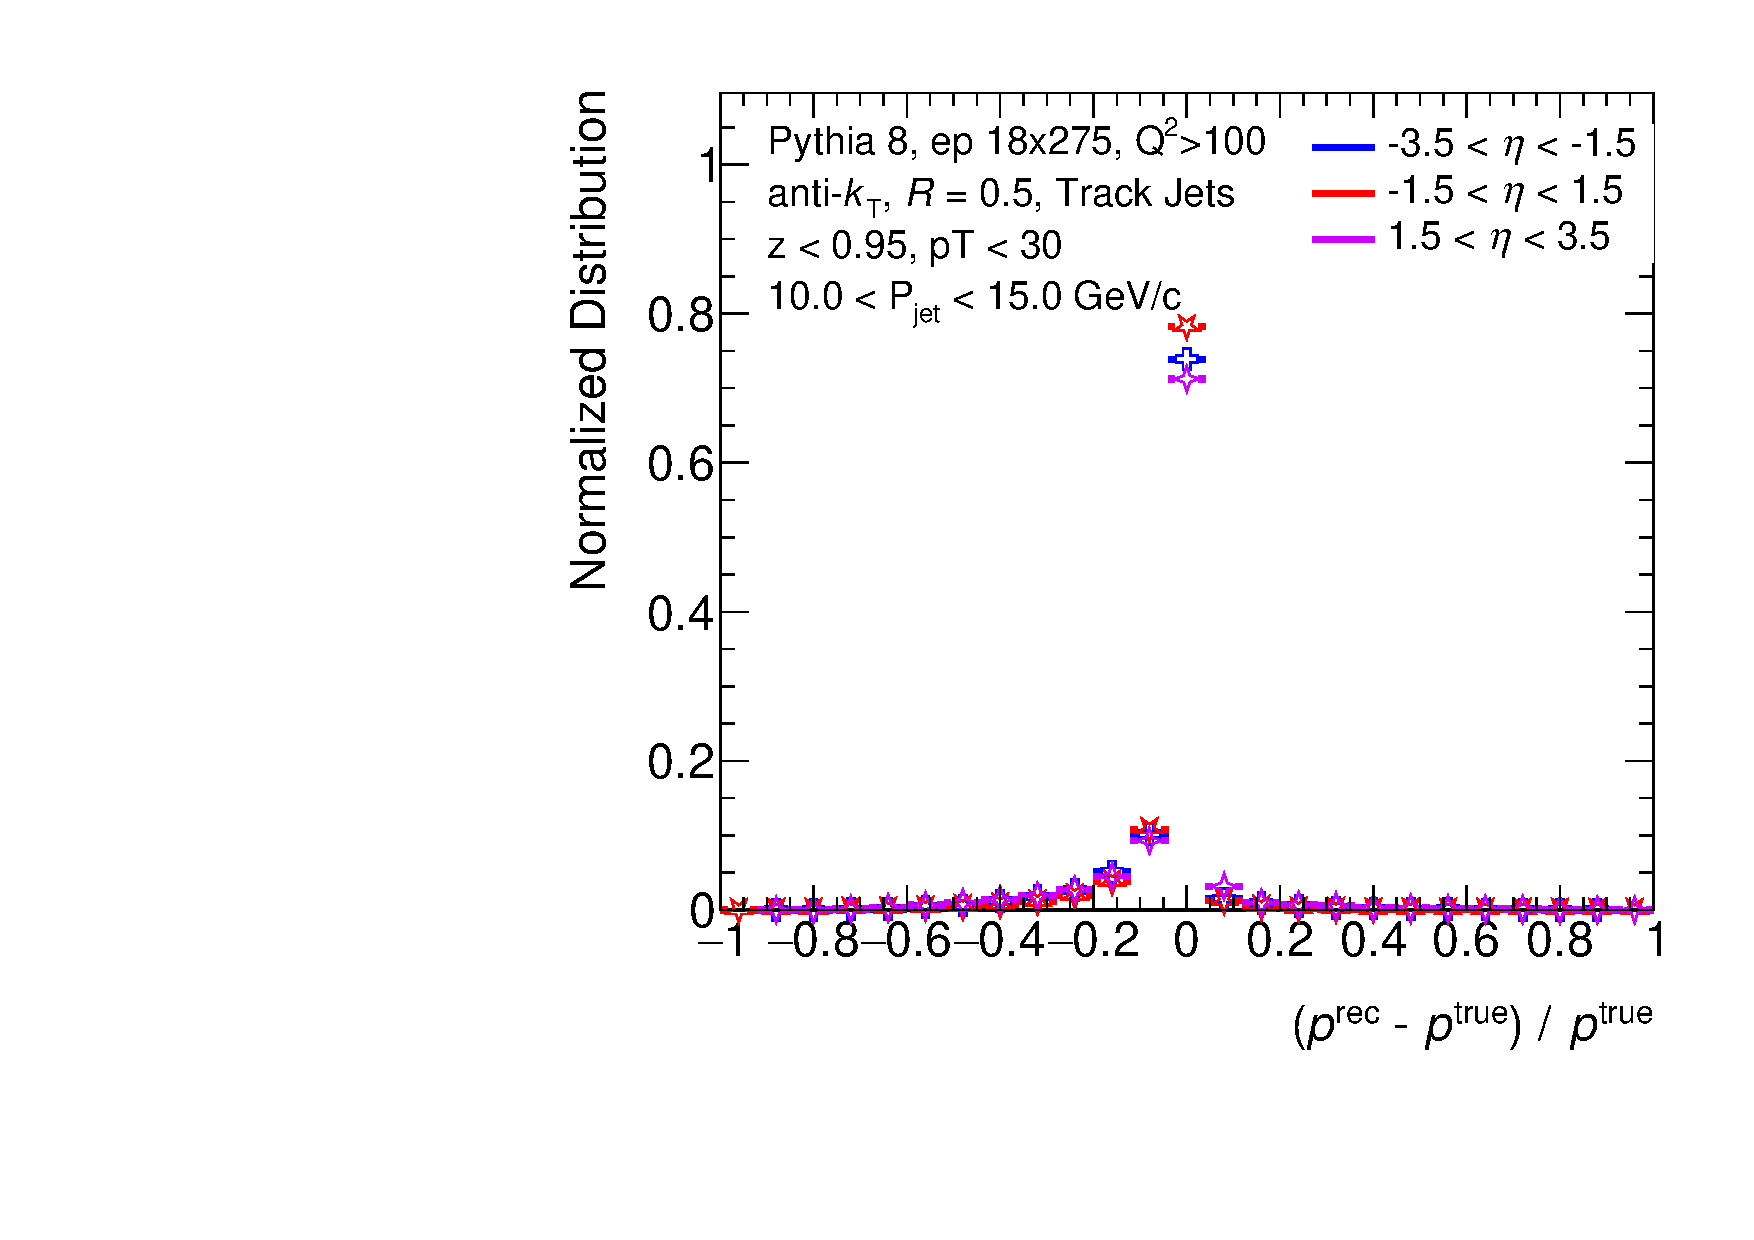
\includegraphics[width=0.6\textwidth]{figs/Final_Plots/JES_Slice_Plot_EtaBins2_grouped.pdf}
    \caption{The distribution of the difference between the true and reconstructed momentum for track jets with a true momentum between 10 and 15 GeV/c.  The mean of the distribution determines the momentum scale of the detector, and the standard deviation of the distribution dictates the resolution.}
    \label{fig:track_momentum_slice}
\end{figure}

The scale and resolution is extracted from the distribution of 

\begin{equation}
    \frac{O^{\hbox{reconstructed}}-O^{\hbox{truth}}}{O^{\hbox{truth}}}
    \label{eq:distribution}
\end{equation}
for energy and momentum, and 
\begin{equation}
    O^{\hbox{reconstructed}}-O^{\hbox{truth}}
    \label{eq:distribution}
\end{equation}

for spatial variables, where $O$ is the observable.  From this distribution, the mean and standard deviation are calculated, corresponding to the scale and resolution respectively of the observable.  To study the response as a function of energy, the spectra was broken into 5 GeV bins, and the scale and resolution calculated for each.  An example of the 10-15 GeV/c bin for tracked jet momentum is shown in figure \ref{fig:track_momentum_slice}.




% Track jet momentum scale and resolution
\begin{figure}[h]
    \centering
    \begin{subfigure}{0.4\textwidth}
        \centering
        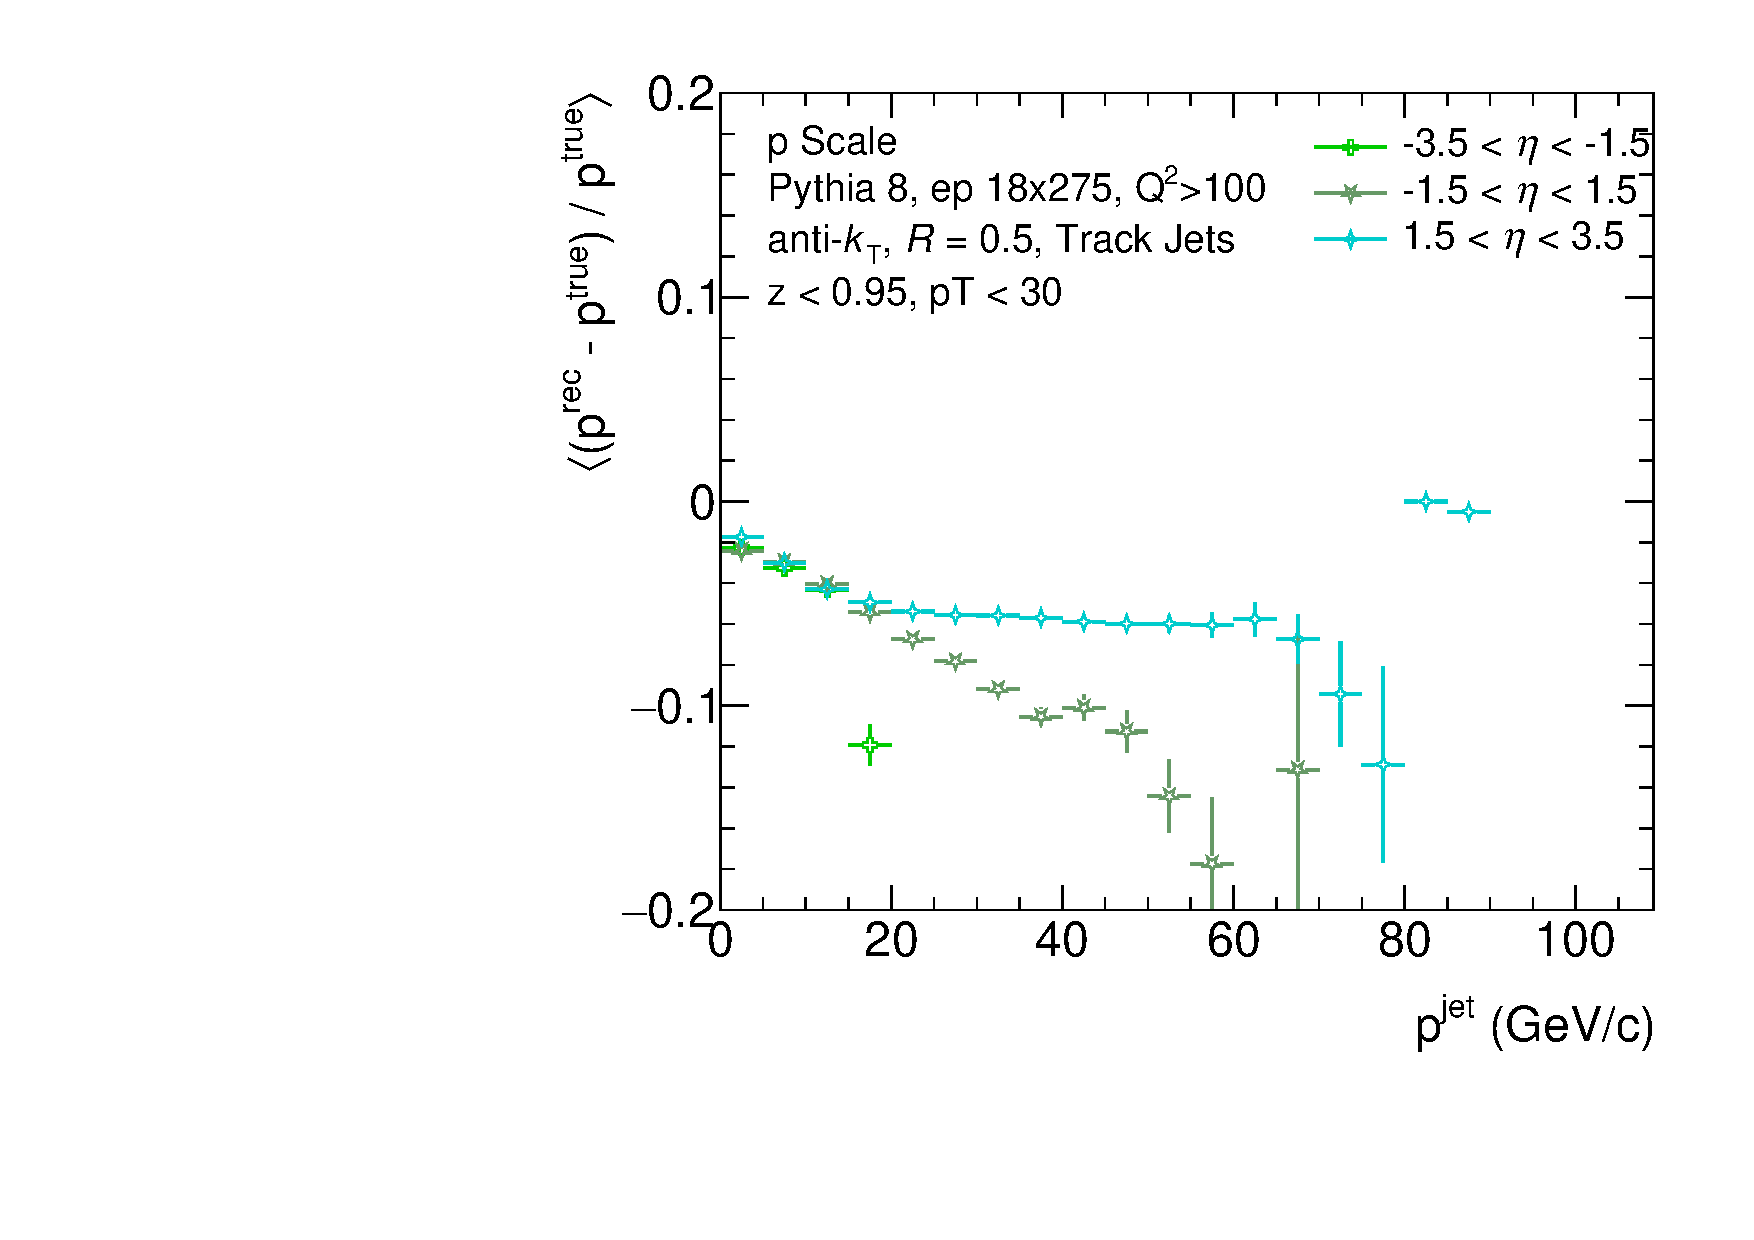
\includegraphics[width=\linewidth]{figs/Final_Plots/pScale_track_grouped.pdf}
        \caption{Track jets scale.  The scale is a measure of how much of the momentum of a truth track was reconstructed.  If all the momentum was measured, the scale would be 0, which is the ideal case.  The scale shown is still very good, and as long as it is well characterized it can be corrected for with calibrations.  }
        \label{fig:track_momentum_scale}
    \end{subfigure}
    \hfill
    \begin{subfigure}{0.4\textwidth}
        \centering
        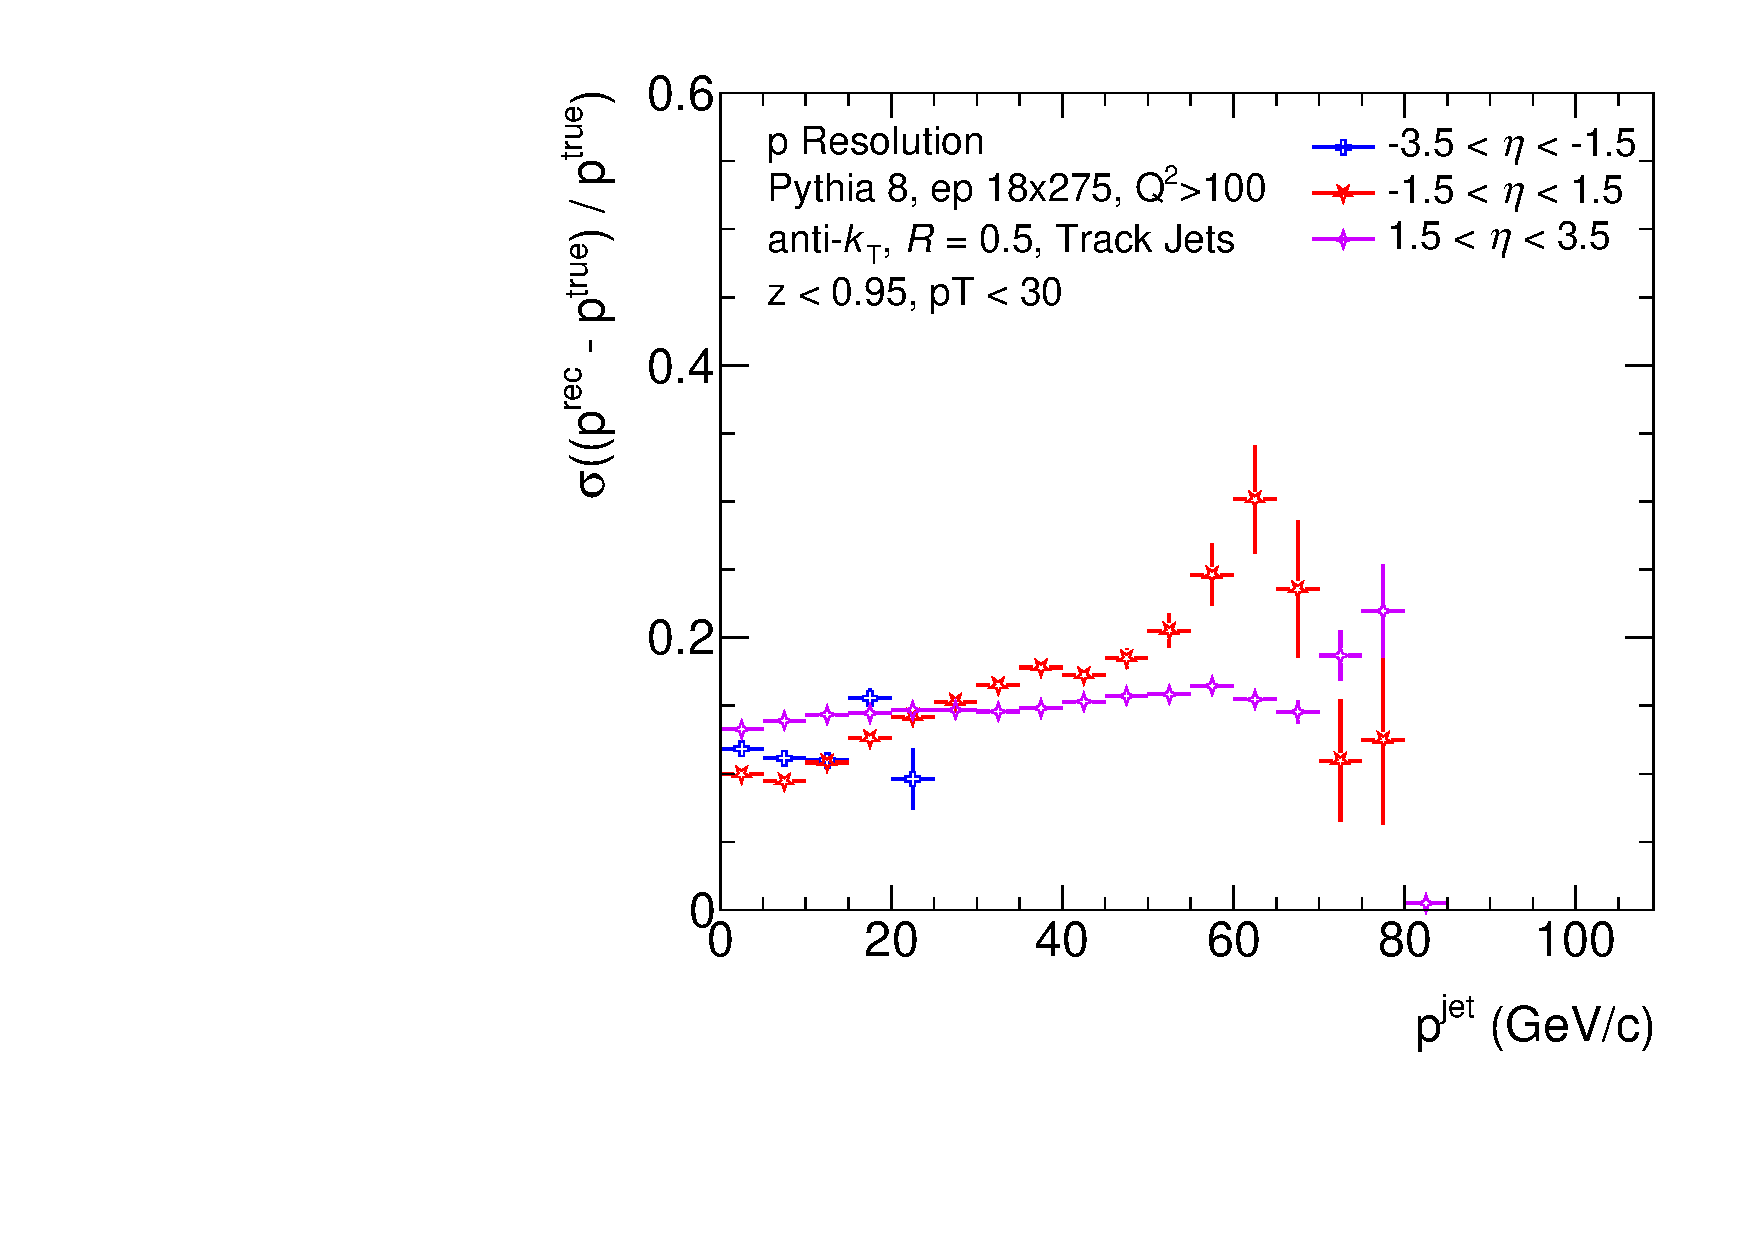
\includegraphics[width=\linewidth]{figs/Final_Plots/pReso_track_grouped.pdf}
        \caption{Track jet resolution.  The resolution is the standard deviation of the spectra of reconstructed jet momentum for a particular truth energy.  The closer the value to zero, the more confidence we have that the value is as measured.  For track jets, we anticipate the resolution to get worse as we go up in momentum, since it becomes harder for the tracking system to distinguish the momentum of the track.}
        \label{fig:track_momentum_resolution}
    \end{subfigure}
    \caption{The scale and resolution of the momentum of track jets.}
    \label{fig:track_momentum_reso_scale}
\end{figure}

As seen in figure \ref{fig:track_momentum_scale}, the jet momentum scale is better than -0.15 across entire detectors acceptance.  This, in combination with the momentum resolution better than 0.2 as shown in figure \ref{fig:track_momentum_resolution} opens up the ability to study charged jets in great detail, especially those with a momentum below 50 GeV/c.  

% Track jet spatial resolution
\begin{figure}[H]
    \centering
    \begin{subfigure}{0.4\textwidth}
        \centering
        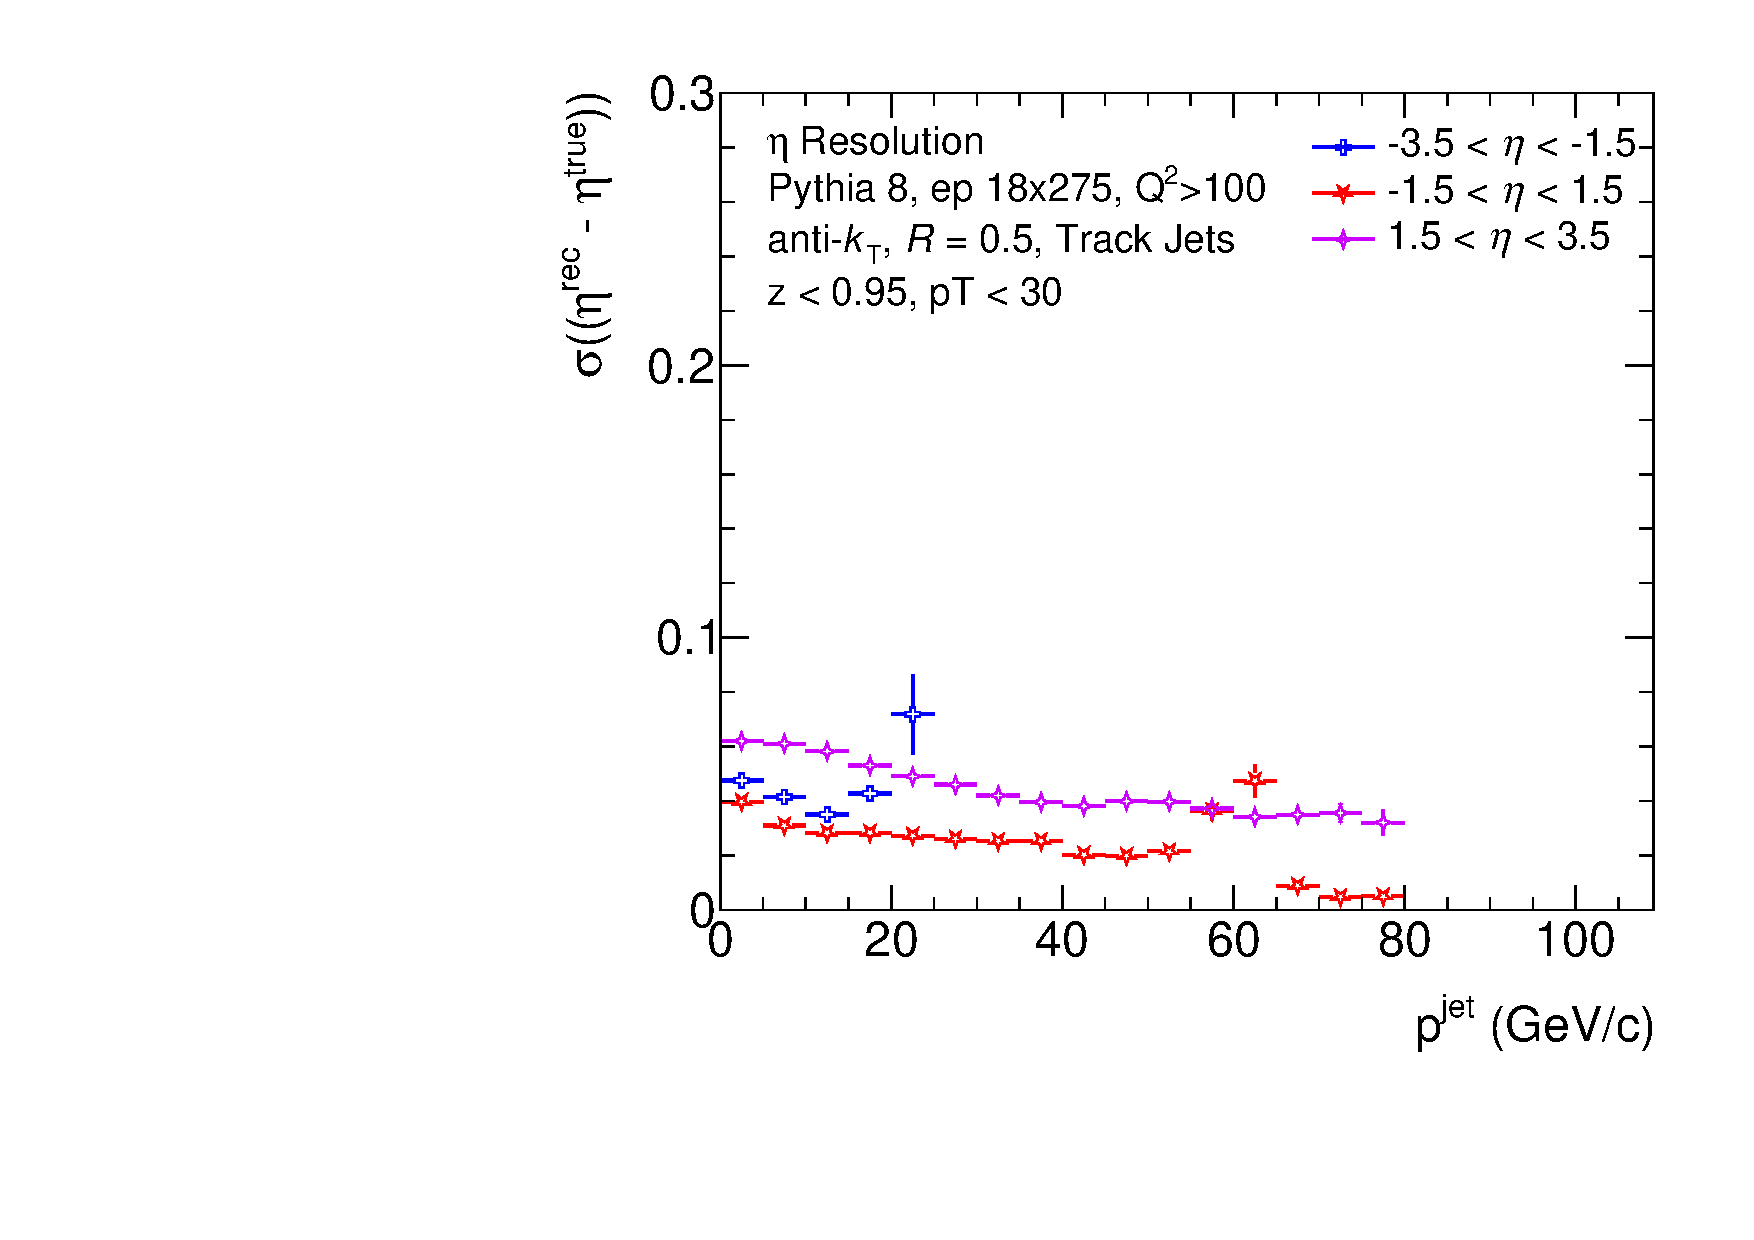
\includegraphics[width=\linewidth]{figs/Final_Plots/EtaReso_track_grouped.pdf}
        \caption{Track jet $\eta$ resolution}
        \label{fig:track_eta_resolution}
    \end{subfigure}
    \hfill
    \begin{subfigure}{0.4\textwidth}
        \centering
        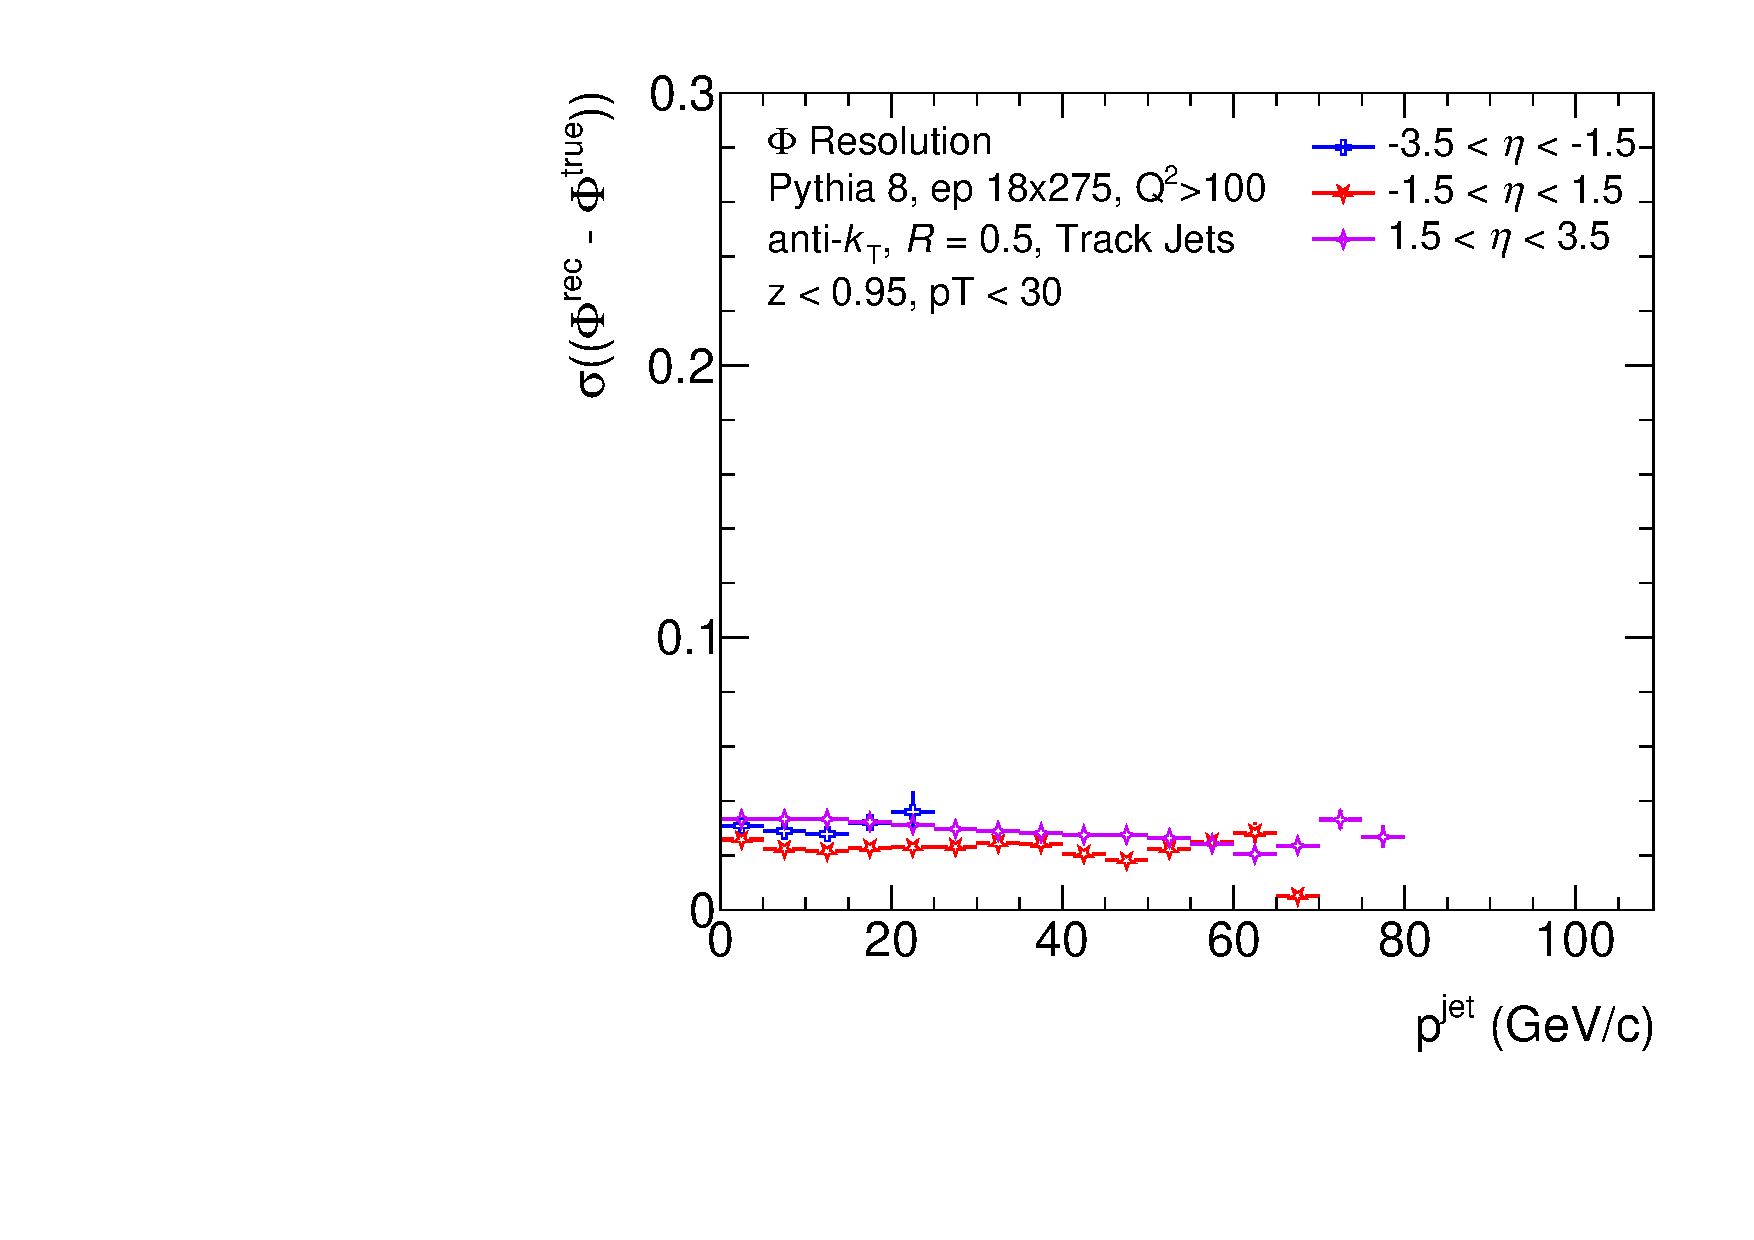
\includegraphics[width=\linewidth]{figs/Final_Plots/PhiReso_track_grouped.pdf}
        \caption{Track jet $\phi$ resolution}
        \label{fig:track_phi_resolution}
    \end{subfigure}
    \caption{The spatial resolution of track jets.  The resolution in both pseudorapidity and azimuthal angle is very good, which is important for correlating jets to the scattered electron for studying parton kinematics.  }
    \label{fig:track_spatial_reso_scale}
\end{figure}

In addition to the excellent momentum scale and resolution the ECCE tracking system offers, the detector offers very good spatial resolution of jets (Figure \ref{fig:track_spatial_reso_scale}).
